\PassOptionsToPackage{pdftex}{graphicx} % pdftex hack fuer graphicx
\documentclass[pdftex,hyperref=pdftex,12pt,aspectratio=169]{beamer}
%\usetheme[fakultaet-oder-cau]{CAU2013}
\usepackage[style=authoryear,citestyle=authoryear,backend=biber]{biblatex}
\addbibresource{references.bib}

\renewcommand{\bibfont}{\ttfamily}

\usepackage{listings}

\usepackage[utf8]{inputenc}
\usepackage[T1]{fontenc}
\usepackage[american]{babel}
\usepackage{csquotes}
\usepackage{mathabx}

\usepackage[scaled=0.8]{beramono}

\usepackage{todonotes}
\usepackage{multicol}
\usepackage{xcolor}
\newcommand\mynote[1]{\textcolor{red}{#1}}
%\usepackage[notocbib]{apacite}

%% Beamer Bibliography Fix
%\def\newblock{\hskip .11em plus .33em minus .07em}
%\bibliographystyle{alpha}

\makeatletter

\makeatother

%% title setup

\title{Course-Software-Testing}
\subtitle{MarDATA} 
\author[Prigge, Rath, Hiremath, Gundlach]{Enno Prigge \and Willi Rath \and Dilip Hiremath \and Sven Gundlach\\[3mm]
Kiel University
}
\date[18-11-2020]{18\textsuperscript{th} November 2020}

%% language settings
\selectlanguage{american}

\begin{document}

%% remove Figure from caption
\setbeamertemplate{caption}{\raggedright\insertcaption\par}

%\ttfamily

% -----------------------------------------

%% make titleslide
{
\begin{frame}[plain]{}{}%
\titlepage
\begin{pgfpicture}{0cm}{0cm}{\textwidth}{1cm}
\pgfline{\pgfxy(0,0)}{\pgfxy(15.5,0)}
\pgfputat{\pgfxy(0,-0.2)}{\pgfbox[left,top]{\pgfimage[width=25mm]{images/MarDATA_logo}}}
\pgfputat{\pgfxy(5.8,-0.1)}{\pgfbox[left,top]{
% \begin{minipage}{95mm}
% \tiny footer
% \end{minipage}
}}
\end{pgfpicture}
\end{frame}
}

\mysubsection{Kontinuierliche Integration}\label{ssec:ci}

%%%%%%%%%%%%%%%%%%%%%%%%%%%%%%%%%

\begin{frame}
 \frametitle{Neue Features: \glqq Naiver\grqq\ Workflow}
 
Typisches \glqq unstrukturiertes\grqq\ Vorgehen:
\begin{itemize}
	\item Implementierung neuer Features
   \item Aufruf und Test der Features aus Main-Methode, Ausgabe mit \textbf{System.out.println}
   \item Manuelle Pr�fung, ob Ergebnisse korrekt (oder zumindest plausibel) sind
   \item Test-Code in Main-Methode wird sp�ter nicht mehr verwendet
\end{itemize}
 
 \pause
 
Nachteile?
 \begin{itemize}
	 \item Code in Main-Methode, der nicht \glqq dahin geh�rt\grqq
		\item Test-Code wird verworfen, obwohl auch sp�ter noch sinnvoll
		\item Tests werden nicht mehr ausgef�hrt
   \item[$\rightarrow$] Regressionen werden nicht erkannt
\end{itemize}
\end{frame}

%%%%%%%%%%%%%%%%%%%%%%%%%%%%%%%%%

\begin{frame}
\frametitle{Kontinuierliche Integration}
Wozu?
\begin{itemize}
  \item Integrations-Probleme werden kontinuierlich entdeckt.
  \item Fr�he Warnungen bei nicht zusammenpassenden Komponenten.
  \item Regressions-Tests entdecken Fehler.
  \item Die Entwickler werden zu einem verantwortlichen Umgang "`erzogen"'.
  \item Beispiel-Werkzeug:
  \begin{itemize}
	\item Jenkins \url{http://jenkins-ci.org/}
  \end{itemize}
\end{itemize}

\vfill

Siehe auch die Vorlesungen zu kontinuierlicher Integration f�r Kieker/ExplorViz und bei PPI.
\end{frame}

%%%%%%%%%%%%%%%%%%%%%%%%%%%%%%%%%

\begin{frame}
\frametitle{Continuous Integration Environment}
\framesubtitle{\tiny http://www.heise.de/developer/artikel/Continuous-Integration-in-Zeiten-agiler-Programmierung-1427092.html}
  \begin{center}
  \dgrafik{\textwidth}{0.3\textwidth}{Konfigurationsmanagement/abbildungen/ContinuousIntegrationEnvironment}
  \end{center}
\end{frame}

%%%%%%%%%%%%%%%%%%%%%%%%%%%%%%%%%

\mysubsubsection{Automatisiertes Testen}

%%%%%%%%%%%%%%%%%%%%%%%%%%%%%%%%%

\begin{frame}
 \frametitle{Automatisches Testen}
 
 Automatische Tests:
  \begin{itemize}
	 \item Test-Code in eigens daf�r vorgesehenem Projektbereich
		\item Ausf�hrung wie \glqq Main-Methoden\grqq, aber Tool-Unterst�tzung f�r:
		\begin{itemize}
    \item Vergleich mit erwartetem Verhalten
    \item automatische Durchf�hrung aller Tests
    \item Statistiken �ber bestandene, nicht bestandene Tests
   \end{itemize}

\end{itemize}

 \pause
 
Vorteile:
\begin{itemize}
	\item Trennung Funktionalit�t und Tests 
   \item Tests bleiben erhalten
   \item Tests k�nnen regelm��ig, automatisch ausgef�hrt werden\\
      $\rightarrow$ Regressionen werden erkannt
   \item Tests als \glqq Quality Gateway\grqq\ f�r Integration von neuem Code in den Master Branch bzw.\ Master Repository
\end{itemize}
\end{frame}

%%%%%%%%%%%%%%%%%%%%%%%%%%%%%%%%%

\begin{frame}
 \frametitle{Automatisches Testen: JUnit}
 
 
\includegraphics[width=0.8cm]{Konfigurationsmanagement/abbildungen/junit.png}
\begin{itemize}
   \item Erstver�ffentlichung 2000
   \item eclipse-Unterst�tzung seit 2002
   \item Einbinden bsp.~mit Maven
\end{itemize}
\pause
 

\includegraphics[width=0.8cm]{Konfigurationsmanagement/abbildungen/junit.png} in Softwaretechnik:
\begin{itemize}
	\item Struktur und Beispiel in Vorlesung
   \item Details in �bung
   \item Eure Abgaben: JUnit-Tests gefordert (Quality-Gateway bei Korrektur)
\end{itemize}
%https://www.vogella.com/tutorials/JUnit/article.html
\end{frame}

%%%%%%%%%%%%%%%%%%%%%%%%%%%%%%%%%

\begin{frame}[containsverbatim]{Eine Beispiel-Funktion}
\framesubtitle{die getestet werden sollte \dots}
\lstset{language=Java}
\begin{lstlisting}[frame=single]
package com.example.project;

public class Calculator {

	public int add(int a, int b) {
		return a - b;
	}

}
\end{lstlisting}
\begin{flushright}
Schauen wir uns das einmal in eclipse an.
\end{flushright}
\end{frame}

%%%%%%%%%%%%%%%%%%%%%%%%%%%%%%%%%

\begin{frame}[containsverbatim]{Eine Beispiel-Test}
\footnotesize
\lstset{language=Java}
\begin{lstlisting}[frame=single]
package com.example.project;

import static 
         org.junit.jupiter.api.Assertions.assertEquals;
import org.junit.jupiter.api.DisplayName;
import org.junit.jupiter.api.Test;

class MyTest {

	@Test
	@DisplayName("1 + 1 = 2")
	void addsTwoNumbers() {
	   Calculator calculator = new Calculator();
	   assertEquals(2, calculator.add(1, 1),
		                "1 + 1 should equal 2");
	}

}
\end{lstlisting}
%import org.junit.jupiter.params.ParameterizedTest;
%import org.junit.jupiter.params.provider.CsvSource;
	%@ParameterizedTest(name = "{0} + {1} = {2}")
	%@CsvSource({
			%"0,    1,   1",
			%"1,    2,   3",
			%"49,  51, 100",
			%"1,  100, 101"
	%})
	%void add(int first, int second, int expectedResult) {
		%Calculator calculator = new Calculator();
		%assertEquals(expectedResult, calculator.add(first, second),
				%() -> first + " + " + second + " should equal " + expectedResult);
	%}

\begin{flushright}
\tiny
\url{https://github.com/junit-team/junit5-samples/}
\end{flushright}
\end{frame}

%%%%%%%%%%%%%%%%%%%%%%%%%%%%%%%%%

\begin{frame}
 \frametitle{Automatisches Testen: Res�mee}
 
 Evaluation:
 \begin{itemize}
	 \item  Automatische Tests machen kaum zus�tzliche Arbeit!
		\item Helfen, Qualit�tsprobleme fr�h zu erkennen
\end{itemize}
 
\pause
 
Fragen:
\begin{itemize}
	\item Wie viele Tests sollte ich schreiben?
   \item Welche Teile des Programms sollten getestet werden?
   \item Und mit welchen Beispieldaten?
   \item Woher wei� ich die \glqq erwarteten\grqq\ Ausgaben?
   \item \dots
\end{itemize}

\pause
 
Mehr dazu im Abschnitt \glqq Qualit�tssicherung\grqq.
\end{frame}

%%%%%%%%%%%%%%%%%%%%%%%%%%%%%%%%%

\mysubsubsection{Mocking}

%%%%%%%%%%%%%%%%%%%%%%%%%%%%%%%%

\begin{frame}[allowframebreaks]
 \frametitle{Mocking: Motivation}
 
Unit Testing:
\begin{itemize}
   \item Code verwendet andere Objekte des Systems
   \item Objekte m�ssen f�r Test verf�gbar sein
\end{itemize}
Schwierigkeiten:
 \begin{itemize}
	   \item Unit-Testing! Kein komplettes System starten!
		 \item Andere Objekte / Klassen eventuell noch nicht verf�gbar!
		 \item Performance
    \item Echtes Objekt schwierig bereitzustellen:
    \begin{itemize}
     \item Spezifische Werte (Uhrzeit, Sensorwerte)
     \item Fehlerzust�nde (Netzwerkfehler, \dots)
    \end{itemize}
\end{itemize}

 \pause 
Beispiele:
\begin{itemize}
	 \item Time-Server
   \item Datenbank
   \item Temperatur-Sensor
   \item Netzwerkdienste
\end{itemize}

Mocking ist insbesondere f�r \glqq Test Driven Development\grqq\ relevant.
\end{frame}

%%%%%%%%%%%%%%%%%%%%%%%%%%%%%%%%%

\begin{frame}
 \frametitle{Ansatz: Mock-Objekte}
 
Alternative: Mock-Objekte (auch: Test Double):
\begin{itemize}
	 \item Objekte, die echtes Verhalten nachahmen
   \item K�nnen im Test anstelle des echten Objekts verwendet werden
\end{itemize}
 
\pause

Interface: 
\begin{itemize}
	 \item M�ssen anstelle des \glqq echten Objekts\grqq\ verwendet werden k�nnen\\
		$\rightarrow$ Gleiches Interface (oder Teilmenge) wie echtes Objekt
\end{itemize}
\pause
 
Verhalten:
\begin{itemize}
	 \item \glqq Angelehnt\grqq\ an echtes Objekt\\
		$\rightarrow$ f�r zu testenden Code: wie echtes Objekt
		\item Explizites Herbeif�hren von Werten, Zust�nden, \dots\\
   $\rightarrow$ f�r Test-Code:\\ konfigurierbar!
\end{itemize}
\end{frame}

%%%%%%%%%%%%%%%%%%%%%%%%%%%%%%%%%

\begin{frame}
 \frametitle{Mock-Objekte: Spektrum}
 
Einfachste Version: Stub-Objekte
\begin{itemize}
	\item Liefert immer feste Antworten auf Anfragen
  \item Antworten k�nnen eventuell vom Test-Code gesetzt werden
\end{itemize}

 \dots
 \pause
 
Komplexeste Version: Fake-Objekte
\begin{itemize}
	\item Funktionierende Implementierung
  \item Einfacher als tats�chlich verwendetes Objekt
\end{itemize}
\end{frame}

%%%%%%%%%%%%%%%%%%%%%%%%%%%%%%%%%

\begin{frame}
 \frametitle{Mock-Objekte: Kategorien}
  \framesubtitle{\url{https://martinfowler.com/articles/mocksArentStubs.html}}
 
 \begin{description}[Dummy objects]
  \item[Dummy objects] are passed around but never actually used. Usually they are just used to fill parameter lists. \pause
  \item[Fake objects] actually have working implementations, but usually take some shortcut which makes them not suitable for production (an in-memory database is a good example). \pause
  \item[Stubs] provide canned answers to calls made during the test, usually not responding at all to anything outside what's programmed in for the test. \pause
  \item[Spies] are stubs that also record some information based on how they were called. \pause
  \item[Mocks] are [\dots] objects pre-programmed with expectations which form a specification of the calls they are expected to receive.
 \end{description}
\end{frame}

%%%%%%%%%%%%%%%%%%%%%%%%%%%%%%%%%

\begin{frame}
 \frametitle{Framework: Mockito}
 
�bersicht:
\begin{itemize}
	\item \url{https://site.mockito.org/}
   \item Java-Framework zum Erstellen von Mock-Objekten
   \item Erste Version: 2008
\end{itemize}

If you use Mockito in tests you typically:
\begin{enumerate}
	\item Mock away external dependencies and insert the mocks into the code under test
	\item Execute the code under test
	\item Verify that the code executed correctly
\end{enumerate}
For example, you can verify that a method has been called with certain parameters. This kind of testing is sometimes called behavior testing. Behavior testing does not check the result of a method call, but it checks that a method is called with the right parameters.
\end{frame}

%%%%%%%%%%%%%%%%%%%%%%%%%%%%%%%%%

\begin{frame}[containsverbatim,allowframebreaks]
 \frametitle{Mockito mit JUnit}
\footnotesize
\lstset{language=Java}
\begin{lstlisting}[frame=single]
import static org.mockito.Mockito.*;

public class MockitoTest  {

  @Mock
  MyDatabase databaseMock;                         // 1

  @Rule public MockitoRule mockitoRule
		            = MockitoJUnit.rule(); // 2

  @Test
  public void testQuery()  {
    ClassToTest t = new ClassToTest(databaseMock); // 3
    boolean check = t.query("* from t");           // 4
    assertTrue(check);                             // 5
    verify(databaseMock).query("* from t");        // 6
  }
}
\end{lstlisting}
\newpage
\normalsize
\begin{enumerate}
	\item Tells Mockito to mock the databaseMock instance
	\item Tells Mockito to create the mocks based on the \texttt{@Mock} annotation
	\item Instantiates the class under test using the created mock
	\item Executes some code of the class under test
	\item Asserts that the method call returned true
	\item Verify that the query method was called on the \texttt{MyDatabase} mock
\end{enumerate}

Siehe auch \url{https://www.vogella.com/tutorials/Mockito/article.html}
\end{frame}

%%%%%%%%%%%%%%%%%%%%%%%%%%%%%%%%%

\begin{frame}
 \frametitle{Mocking: Res�mee}
 
Motivation: Komplexe Objekte f�r Test \glqq ersetzen\grqq:
\begin{itemize}
  	\item Simulieren
    \item Durch Dummies ersetzen
    \item Zus�tzlich Aufruf-Informationen sammeln
\end{itemize}
Verh�ltnis zu Unit-Testing:
\begin{itemize}
	 \item Erg�nzt assertions durch Verification: Testen von Interaktionen mit dem Mock-Objekt
\end{itemize}
Verifikation:
\begin{itemize}
	\item Mock-Objekte speichern Aufrufinformationen. Dies erlaubt eine �berpr�fung von Eigenschaften der \textit{Aufruf-History} der Mock-Objekte
  \item \textbf{Achtung}: Nicht verwechseln mit formaler Verifikation!
\end{itemize}
Unit Tests \textit{vs.} Mock-Verification?
\begin{itemize}
	\item Erg�nzung, nicht Ersatz: �berpr�fen unterschiedliche Aspekte!
  \item \textbf{Mehr Details und Beispiele: �bung!}
\end{itemize}
\end{frame}


\begin{frame}
 \frametitle{Quality control: Overview}

Quality control for software:
\begin{itemize}
  \item Known: Software errors occur in practice.
  \item Goal: Prevent errors \textbf{at least} in live software.
\end{itemize}
Options?
 \pause
\begin{itemize}
  \item Code Review
   \begin{itemize}
    \item four-eyes principle
    \item Team Review, if applicable via pair programming
   \end{itemize} \pause
  \item Tests
   \begin{itemize}
    \item Manually
    \item Automatically
   \end{itemize} \pause
  \item Formal methods
   \begin{itemize}
    \item Formal verification
    \item Proofs of Program Correctness 
   \end{itemize}
\end{itemize}
\end{frame}

%%%%%%%%%%%%%%%%%%%%%%%%%%%%%%%%%

\begin{frame}
\frametitle{Things we do not want: Bugs}
%\framesubtitle{\citep{Binder1999}}
  \begin{center}
  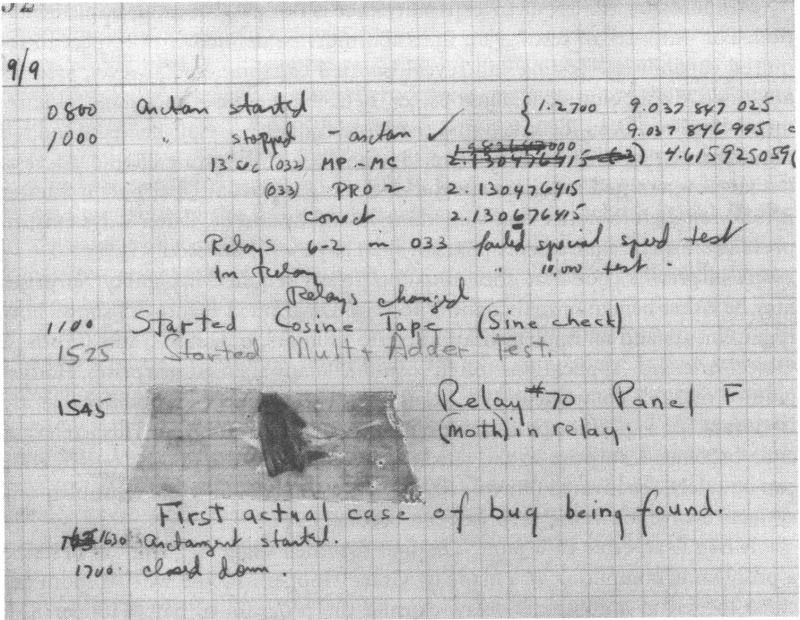
\includegraphics[width=.85\textwidth]{images/Qualitaetssicherung/abbildungen/Bug}
  \end{center}

\end{frame}

%%%%%%%%%%%%%%%%%%%%%%%%%%%%%%%%%

\section{Validation \& Verification}

%%%%%%%%%%%%%%%%%%%%%%%%%%%%%%%%%

\begin{frame}
\frametitle{Validation and verification of software}
\begin{itemize}
  \item Validation and verification of the implemented software system:%\citep{Boehm1984,FisherVV2007}:
    \begin{itemize}
      \item "`Do we build the system right?"' (Verification)\\
            Check  that the system meets the requirements
      \item "`Do we build the right system?"' (Validation)\\
            Check whether the \emph{actual} (user) requirements have been realized.
    \end{itemize}
  \item Validation can be supported e.g. by prototyping (see LE \ref{sec:Process_Models})
  \item Occasionally these terms are also used differently:
    \begin{itemize}
      \item e.g. verification for formal proofs and validation for \emph{running}.
    \end{itemize}
\end{itemize}
\end{frame}

%%%%%%%%%%%%%%%%%%%%%%%%%%%%%%%%%

\begin{frame}\frametitle{Validation and Verification: Roles}
\begin{center}
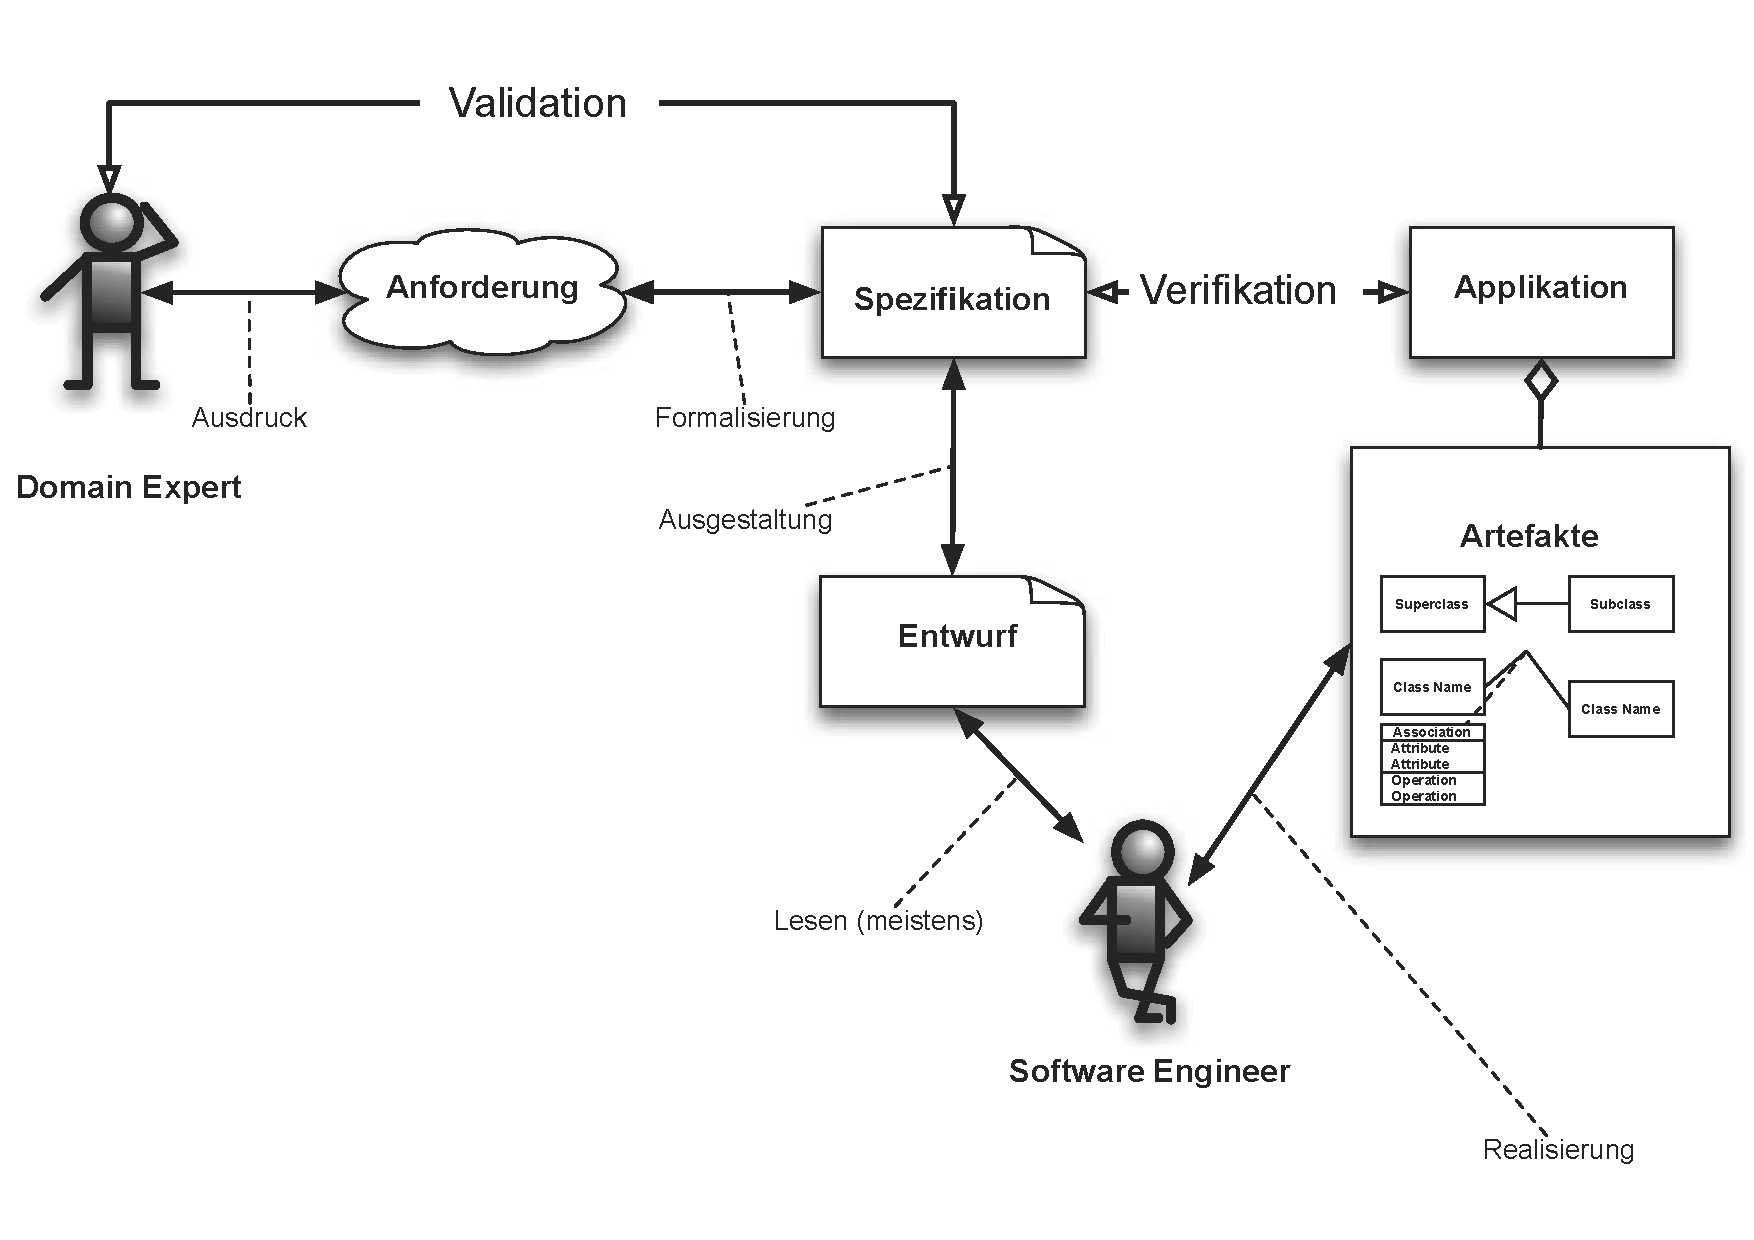
\includegraphics[width=\textwidth]{images/Qualitaetssicherung/abbildungen/ValidationVerifikation}
\end{center}
\end{frame}

%%%%%%%%%%%%%%%%%%%%%%%%%%%%%%%%%

\begin{frame}
\frametitle{Verification Objectives}
\begin{itemize}
  \item Proof of the correct functioning of all functions of a system in relation to a given specification
    \begin{itemize}
      \item Identify errors
      \item Absence of errors
    \end{itemize}
  \item The verification process itself must also be verified: 
    \begin{itemize}
      \item Are the test conditions correct?
      \item Is a formal proof correct? 
    \end{itemize}
  \item Technical (non-functional) requirements must also be checked:
    \begin{itemize}
      \item Efficiency, portability, modifiability, etc.
    \end{itemize}
  \item The result is not always simply \emph{correct} or \emph{incorrect}.
    \begin{itemize}
      \item Reliability requirements and subjectivity require more fine-grained metrics,\\
      e.g. \emph{good enough} or 99\% availability.
    \end{itemize}
\end{itemize}
\end{frame}



%%%%%%%%%%%%%%%%%%%%%%%%%%%%%%%%%

\begin{frame}
\frametitle{Classification of verification techniques}

\begin{block}{Symbolic Execution}
The behavior of the system is tested with respect to the expected behavior.
\begin{itemize}
  \item Structure-oriented methods\\
        white-box, with knowledge of the implementation 
  \item Function-oriented methods\\
        black-box, without knowledge of the implementation
\end{itemize}
\end{block}
%Verification https://www.researchgate.net/figure/Classification-of-verification-techniques_fig3_36374045
%veritesting https://dl.acm.org/doi/abs/10.1145/2568225.2568293
%white-box fuzz testing http://pxzhang.cn/paper/concolic_testing/FuzzTesting.pdf
%concolic testing https://dl.acm.org/doi/abs/10.1145/1065010.1065036
 
\vspace{1ex}
\begin{block}{Static Analysis}
The behavior of a system is analyzed to derive whether the behavior is correct.
\begin{itemize}
  \item Static proofs of correctness
  \item Reviews, inspections, walkthroughs, etc.
\end{itemize}
\end{block}
\end{frame}

%%%%%%%%%%%%%%%%%%%%%%%%%%%%%%%%%
\subsection{Testing}

\begin{frame}
\frametitle{Testing for verification}
\begin{description}[Integration test]
  \item[Unit-Test]
  Single functions / components are tested.
  \item[Integration test]
  Interdependent components are tested together.\\
            Focus on interface testing.\\
        Components are integrated into subsystems and tested together.
  \item[System test]
  Test of the complete system.
\end{description}  
\begin{block}{Objective of a test planning}
Select test cases in such a way that the probability of finding errors or ruling them out is high.
\end{block}
\end{frame}

%%%%%%%%%%%%%%%%%%%%%%%%%%%%%%%%%

\begin{frame}
\frametitle{The V-Model}
\framesubtitle{Use especially by military and governmental authorities.}
\begin{center}
\pgfimage[width=\textwidth]{images/Qualitaetssicherung/abbildungen/VModel}
\end{center}
Verification and validation of the sub-products are essential components of the V-Model.
\end{frame}
%https://www.researchgate.net/figure/V-model-for-software-development_fig2_36374045

%%%%%%%%%%%%%%%%%%%%%%%%%%%%%%%%%

\begin{frame}
\frametitle{Problems in software testing}
\begin{itemize}
  \item Test cases often describe the behavior more detailed than the specification: 
    \begin{itemize}
      \item[$\rightarrow$] Develop test cases before implementation
    \end{itemize}
  \item Basic problem: \\
        ``Program testing can be used to show the presence of bugs, but never to show their absence.'' %\citep{Dijkstra72}
  \item Questions to answer:
   \begin{itemize}
  	\item How to determine suitable test cases and test plans? 
    \item How to check the correctness of the test implementation? 
    \item Who is the tests authority? 
   \end{itemize}
\end{itemize}
\end{frame}

%%%%%%%%%%%%%%%%%%%%%%%%%%%%%%%%%

%\begin{frame}
%\frametitle{The test process}
%\framesubtitle{\citep{Sommerville2018}}
  %\begin{center}
  %\includegraphics[width=1.05\textwidth]{images/Qualitaetssicherung/abbildungen/TestProcess}
  %\end{center}
%This represents a possible test process oriented to the V-Model.
%\end{frame}

%%%%%%%%%%%%%%%%%%%%%%%%%%%%%%%%%

\begin{frame}
\frametitle{Challenges of the steps in the test process}
    \begin{itemize}
    \item Identification of test scenarios (use cases)
         \begin{itemize}\item What is to be tested?
         \end{itemize} 
    \item Establishment of concrete test scenarios
          \begin{itemize}
           \item How is the test candidate executed?
           \item What is the correct behavior?
          \end{itemize} 
    \item Formalization of tests 
         \begin{itemize}\item How is the test specified? 
         \end{itemize} 
    \item Carrying out tests 
         \begin{itemize}\item Automation!
         \end{itemize} 
    \item Maintenance of tests
         \begin{itemize}\item Synchronized with the changes in the business software, the tests must (mostly) be adapted and modified.
         \end{itemize} 
    \end{itemize}
\end{frame}

%%%%%%%%%%%%%%%%%%%%%%%%%%%%%%%%%

\begin{frame}
\frametitle{Objectives for software testing}
\begin{itemize}
  \item It must be clear what results are expected when testing.
  \item Use of \emph{systematic} methods:
    \begin{itemize}
      \item Selection of test cases if possible not (only) intuitive or random.
    \end{itemize}
  \item The results should be fully reproducible. 
    \begin{itemize}
      \item This is a major problem especially when testing parallel programs.
    \end{itemize}
  \item Errors should not only be detected, but also localized and fixed. %\citep{Rohr2007}.
    \begin{itemize}
      \item \glq Known bugs\grq\ are not a sign of high quality software.
    \end{itemize}       
  \item Quality requirements must be checked with the highest accuracy possible.
\end{itemize}
\end{frame}

%%%%%%%%%%%%%%%%%%%%%%%%%%%%%%%%%

\begin{frame}
\frametitle{Pragmatic view on testing}
\begin{itemize}
    \item Testing allows conclusions about the quality of a software system 
    \item Quantitative metrics support conclusions 
         \begin{itemize}\item Test coverage etc. 
         \end{itemize} 
    \item Automated regression tests provide protection against side effects of modifications 
		\begin{itemize}
			\item A regression test is the repetition of test cases to ensure that modifications in already tested parts of the software do not cause new errors (``regressions''). 
		\end{itemize}
\end{itemize}
\end{frame}

%%%%%%%%%%%%%%%%%%%%%%%%%%%%%%%%%

\begin{frame}
\frametitle{Black-Box vs. White-Box Testing}
  \begin{center}
  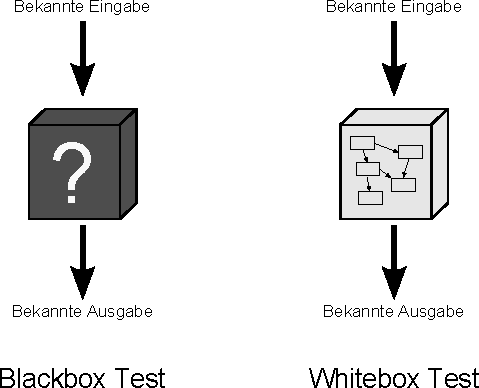
\includegraphics[width=.8\textwidth]{images/Qualitaetssicherung/abbildungen/BlackBoxAndWhiteBoxTesting}
  \end{center}
\end{frame}


\mysubsubsection{White-Box Testen}

%%%%%%%%%%%%%%%%%%%%%%%%%%%%%%%%%

\begin{frame}
\frametitle{White-box Testen von Modulen}
\framesubtitle{(testing in the small)}
\begin{description}[Anwei]
  \item[C0: Anweisungs�berdeckung:] Jede Anweisung soll durch eine geeignete Testmenge mindestens einmal durchlaufen werden (Anweisungs�berdeckungskriterium).
  \item[C1: Kanten�berdeckung:] Jede Kante eines Kontrollflussgraphen soll mindestens einmal durchlaufen werden (Kanten�berdeckungskriterium).
  \item[C2: Pfad�berdeckung:] Jeder Pfad vom Start- zum Endknoten soll durch eine geeignete Testmenge mindestens einmal durchlaufen werden (Pfad�berdeckungskriterium).
  \item[C3: Bedingungs�berdeckung:] Jede m�gliche Kombination der Teilbedingungen muss mindestens einmal durchlaufen werden (Bedingungs�berdeckungskriterium).
\end{description}
\end{frame}

%%%%%%%%%%%%%%%%%%%%%%%%%%%%%%%%%

\begin{frame}
\frametitle{Probleme mit der Anweisungs�berdeckung}
\framesubtitle{C0: Anweisungs�berdeckung}
\begin{itemize}
  \item Ist ein Programm ausreichend getestet, wenn jede Anweisung mindestens einmal ausgef�hrt wurde?
  \item Wie bestimmt man eine minimale Testmenge? 
  \item Ist es sinnvoll, auch leere Anweisungen (z.B. fehlendes \texttt{else}) zu �berdecken? 
  \item Die Struktur des Programms bleibt unber�cksichtigt 
  \item Grunds�tzlich:\\
        �berdeckung ist nicht entscheidbar!
\end{itemize}
\end{frame}

%%%%%%%%%%%%%%%%%%%%%%%%%%%%%%%%%

\begin{frame}
\frametitle{�berdeckung aller Kanten eines Kontrollflussgraphen}
\framesubtitle{C1: Kanten�berdeckung}
Voraussetzung ist die Konstruktion eines Kontrollflussgraphen f�r ein (imperatives) Programm:
\begin{itemize}
  \item Jede einfache Anweisung, die keine weiteren Anweisungen enth�lt, wird als Knoten dargestellt.
  \item Bedingte Anweisungen werden als Verzweigungen dargestellt.
  \item Schleifen werden als Zyklen und
  \item Sequenzen durch Kanten zwischen Knoten dargestellt.
\end{itemize}
\end{frame}

%%%%%%%%%%%%%%%%%%%%%%%%%%%%%%%%%

\begin{frame}
\frametitle{Konstruktion von Kontrollflussgraphen}
\begin{center}
\pgfimage[width=\textwidth]{Qualitaetssicherung/abbildungen/Kontrollflussgraphen}
\end{center}
\end{frame}

%%%%%%%%%%%%%%%%%%%%%%%%%%%%%%%%%

\begin{frame}[fragile]
\frametitle{Beispiel: Programm zur Fakult�tsberechnung}
\begin{columns}
\begin{column}{0.4\textwidth}
\lstset{language=Java,basicstyle=\small}
\begin{lstlisting}
public long fakultaet
            (int n) {
  if (n < 0) {
    throw new 
      Exception();
  }
  long fak = 1;

  while (n > 0) {
    fak *= n;
    n--;
   }
  return fak;
}
\end{lstlisting}
\end{column}
\pause
\begin{column}{0.6\textwidth}
\begin{center}
\pgfimage[width=\textwidth]{Qualitaetssicherung/abbildungen/Fakultaetsberechnung}
\end{center}
\end{column}
\end{columns}
\end{frame}

%%%%%%%%%%%%%%%%%%%%%%%%%%%%%%%%%

\begin{frame}
\frametitle{Testf�lle zur Kanten�berdeckung}
\begin{tabular}{llp{0.2\textwidth}p{0.18\textwidth}p{0.28\textwidth}}
\textbf{Nr} & \textbf{Klasse} & \textbf{Beschreibung des Testfalls} & \textbf{Erwartetes Ergebnis}  & \textbf{Beispielhafte Eingabedaten} \\
~\\
1           & Normal          & Eingabeparame\-ter ist g�ltig	& Fakult�t des Eingabeparameters	& 42 \\
            & \multicolumn{4}{l}{�berpr�fte Kanten: 2, 3, 4, 5, 6, 7} \\[2em]
2           & Fehler          & Eingabeparame\-ter ist nicht g�ltig   & Exception & -1 \\
            & \multicolumn{4}{l}{�berpr�fte Kanten: 1}
\end{tabular}
\end{frame}

%%%%%%%

\begin{frame}
\frametitle{Zyklomatische Komplexit�t}
\framesubtitle{\citet{McCabe1976,EbertCain2016}}
\begin{itemize}
  \item Hinter dieser Software-Metrik von McCabe steckt der Gedanke, dass ab einer bestimmten Komplexit�t ein Modul f�r Menschen nicht mehr begreifbar ist. 
  \item Die zyklomatische Komplexit�t ist definiert als die Anzahl unabh�ngiger Pfade auf dem Kontrollflussgraphen eines Moduls.
  \item Die zyklomatische Komplexit�t gibt an, wie viele Testf�lle n�tig sind, um eine Kanten�berdeckung zu erreichen.
	\item Das Komplexit�tsma� nach McCabe ist gleich der Anzahl der bin�ren Verzweigungen plus 1.
	\item Laut McCabe sollte die zyklomatische Zahl eines in sich abgeschlossenen Teilprogramms nicht h�her als 10 sein, da sonst das Programm zu komplex und zu schwer zu testen ist.
\end{itemize}
\end{frame}


\begin{frame}
\frametitle{Zyklomatische Komplexit�t: Beispiel}
\framesubtitle{\citet{McCabe1976,EbertCain2016}}
\begin{columns}
\begin{column}{0.5\textwidth}
\begin{center}
\pgfimage[width=\textwidth]{Qualitaetssicherung/abbildungen/CylomaticComplexity}
\end{center}
\end{column}
\begin{column}{0.5\textwidth}
\pause
Path 1:  1,2,3,6,7,8\\
\pause
Path 2:  1,2,3,5,7,8\\
\pause
Path 3:  1,2,4,7,8\\
\pause
Path 4:  1,2,4,7,2,4,...7,8\\
\bigskip\bigskip
Zyklomatische Komplexit�t = 4
\end{column}
\end{columns}
\end{frame}



%
%%%%%%%%%%%%%%%%%%%%%%%%%%%%%%%%%%
%
%\begin{frame}[fragile]
%\frametitle{Beispiel: Programm zur Sitzplatzreservierung}
%\small
%\begin{verbatim}
%PROCEDURE Sitzplan; 
%BEGIN 
    %If sitzplanliste.aktualisiert = neu  then 
    %BEGIN 
        %While (sitzplanliste <> nil)  do 
        %BEGIN   
            %Case sitzplanliste.sitz.status of 
              %CFrei: platz_ausgeben (frei); 
              %CBelegt: platz_ausgeben (belegt); 
              %CReserviert: platz_ausgeben (reserviert); 
            %END; 
            %sitzplatzliste := sitzplatzliste.next; 
        %END;
        %sitzplanliste.aktualisiert := Caktualisiert; 
    %END 
    %Else 
        %fehlervar := nicht_neu,
%END;
%\end{verbatim}
%\end{frame}
%
%%%%%%%%%%%%%%%%%%%%%%%%%%%%%%%%%%
%
%\begin{frame}
%\frametitle{Kontrollflussdiagramm f�r Sitzplatzreservierung}
%\begin{center}
%\dgrafik{.8\textheight}{.7\textwidth}{Qualitaetssicherung/abbildungen/Sitzplatzreservierung}
%\end{center}
%\end{frame}

%%%%%%%%%%%%%%%%%%%%%%%%%%%%%%%%%

%\begin{frame}
%\frametitle{Testf�lle zur Kanten�berdeckung}
%\begin{tabular}{llp{0.2\textwidth}p{0.18\textwidth}p{0.28\textwidth}}
%\textbf{Nr} & \textbf{Klasse} & \textbf{Beschreibung des Testfalls} & \textbf{Erwartetes Ergebnis}  & \textbf{Beispielhafte Eingabedaten} \\
%1           & Normal          & Sitzplan ist neu                    & Ausgabe des Sitzplanes        & Neuer Sitzplan mit einem freien, einem belegten und einem reservierten Sitz muss als Parameter �bergeben werden. \\
            %& \multicolumn{4}{l}{�berpr�fte Kanten: 1, 4, 5, 6, 7, 8, 9, 10, 11, 12, 13} \\[2em]
%2           & Fehler          & Sitzplan ist alt                    & Setzen der Fehlervariablen    & Sitzplan wurde seit der letzten Verwendung nicht ver�ndert \\
            %& \multicolumn{4}{l}{�berpr�fte Kanten: 2, 3}
%\end{tabular}
%\end{frame}

%%%%%%%%%%%%%%%%%%%%%%%%%%%%%%%%%

\begin{frame}
\frametitle{Anmerkungen zum Kanten�berdeckungskriterium}
\begin{itemize}
  \item Es wird erzwungen, dass jede Bedingung jeweils mit true und false durchlaufen wird.
  \item Das Kanten�berdeckungskriterium ist somit \emph{sch�rfer} als das Anweisungs�berdeckungskriterium.
  \item Gelegentlich jedoch nicht scharf genug:
    \begin{itemize}
      \item Zusammengesetzte Bedingungen werden nicht hinreichend ber�cksichtigt.
    \end{itemize}
  \item Unzureichend f�r den Test von Schleifen
\end{itemize}
\end{frame}

%%%%%%%%%%%%%%%%%%%%%%%%%%%%%%%%%

\begin{frame}[fragile]
\frametitle{Pfad�berdeckung}
\framesubtitle{C2: Pfad�berdeckung}
 Auch bei einfachen Bedingungen kann die Kanten�berdeckung noch unzureichend sein:
\begin{columns}
\begin{column}{0.3\textwidth}
\lstset{language=Java,basicstyle=\small}
\begin{lstlisting}
if (x != 0) {
   y = 5;
}
else {
   y = 6;
}
if (z > 1) {
   z = z / x;
}
else {
   z = 0;
}
\end{lstlisting}
\end{column}
\pause
\begin{column}{0.7\textwidth}
\begin{itemize}
  \item Die Testmenge \{(x=0, z=1), (x=1, z=3)\} erf�llt zwar das Kanten�berdeckungskriterien, erkennt aber nicht die Division durch 0.
  \item Abh�ngigkeiten bleiben unerkannt!
\end{itemize}
\end{column}
\end{columns}
\end{frame}

%%%%%%%%%%%%%%%%%%%%%%%%%%%%%%%%%

\begin{frame}
\frametitle{Pfad�berdeckung (Fortsetzung)}
\begin{itemize}
  \item Die Testmenge\\
   \{(x=0, z=1), (x=1, z=3), (x=0, z=3), (x=1, z=1)\}\\
   erf�llt das Pfad�berdeckungskriterium.
  \item Problem: Die Anzahl der Pfade w�chst exponentiell mit der L�nge des Programmcodes, so dass ein Testen mit dem Pfad�berdeckungskriterium unrealistisch ist.
  \item Weiteres Problem: Anzahl Pfade f�r Schleifen.\\
  L�sungsansatz: Heuristiken.\\
   Beispielheuristik f�r die Anzahl von Schleifendurchl�ufen:
    \begin{itemize}
      \item 0 mal
      \item \emph{mittelm��ig} oft 
      \item maximale Anzahl 
    \end{itemize}
  Grenzwerte sind wichtig!
\end{itemize}
\end{frame}

%%%%%%%%%%%%%%%%%%%%%%%%%%%%%%%%%

\begin{frame}
\frametitle{Bedingungs�berdeckung}
\framesubtitle{C3}
Hierbei wird z.B.\\
%\begin{lstlisting}
\begin{quote}
\texttt\sffamily{if (C1 and C2) ST;\\
~~else SF;}
\end{quote}
in die folgende Anweisung transformiert:\\
\begin{quote}
\texttt\sffamily{if (C1)\\
~~if (C2) ST\\
~~else SF\\
else SF}
\end{quote}

\vspace{\baselineskip}
\begin{itemize}
  \item Der neue Kontrollflussgraph �berdeckt alle elementaren (Teil-)Bedingungen und macht damit \emph{versteckte} Kanten sichtbar.
  \item Das Bedingungs�berdeckungskriterium ergibt somit ggf.\ noch sch�rfere Testmengen.
\end{itemize}
\end{frame}

\subsection{Black-Box Testing}

%%%%%%%%%%%%%%%%%%%%%%%%%%%%%%%%%

\begin{frame}
\frametitle{Black Box vs. White Box Testing}
  % TODO: Translate image
  \begin{center}
  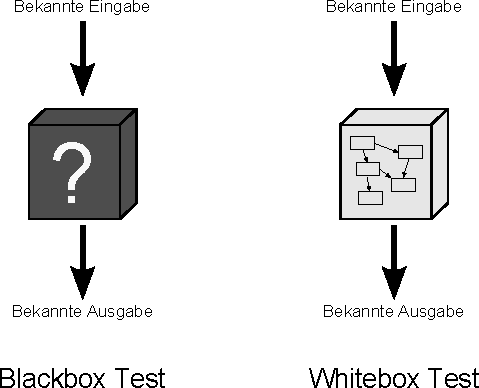
\includegraphics[width=.8\textwidth]{images/Qualitaetssicherung/abbildungen/BlackBoxAndWhiteBoxTesting}
  \end{center}
\end{frame}

%%%%%%%%%%%%%%%%%%%%%%%%%%%%%%%%%

\begin{frame}
\frametitle{Blackbox Testing of modules}
\begin{itemize}
  \item Idea: A part of a program is tested without knowledge of the internal implementation.
  \item Problem: How to define the test set? 
  \item Defining the test set can only rely on the specification.
  \item Formal specifications are then a prerequisite for the systematic generation of test sets.
\end{itemize}
\end{frame}

%%%%%%%%%%%%%%%%%%%%%%%%%%%%%%%%%

\begin{frame}
\frametitle{Medieval Example}
Solutions for equations of the form:
\begin{equation*}
  x^3 + ax^2 + bx + c = 0
\end{equation*}
 
\begin{itemize}
  \item 1535: Tartaglia finds a solutions but keeps it to himself.
  \item Fior poses 30 problems to test this.
  %\item See \citep{Wussing_Arnold1975}
\end{itemize}
\end{frame}

%%%%%%%%%%%%%%%%%%%%%%%%%%%%%%%%%

\begin{frame}
\frametitle{Medieval Black Box Text}
\setlength{\unitlength}{0.1\textwidth}
\begin{center}
\begin{picture}(9,5)
\put(0,5){\makebox(0,0)[tl]{Tartaglia}}
\put(9,5){\makebox(0,0)[tr]{Fior}}
\put(9,4){\makebox(0,0)[tr]{solves $(x-r)(x-s)(x-t)$}}
\put(4.5,3.3){\makebox(0,0){$x^3+ax^2+bx+c = 0$}}
\put(7,3){\vector(-1,0){5}}
\put(4.5,1.8){\makebox(0,0){r', s', t'}}
\put(2,1.5){\vector(1,0){5}}
\put(9,1){\makebox(0,0)[tr]{verifies $r=r', s=s', t=t'$}}
\end{picture}
\end{center}
\end{frame}


%%%%%%%%%%%%%%%%%%%%%%%%%%%%%%%%%
%
%\begin{frame}
%\frametitle{Blackbox Testing}
%\begin{center}
%\hspace*{4em} \pgfimage[width=0.8\textwidth]{images/Qualitaetssicherung/abbildungen/BlackboxTesten}
%\end{center}
%\end{frame}
%
%%%%%%%%%%%%%%%%%%%%%%%%%%%%%%%%%%
%
%\begin{frame}
%\frametitle{Example: Testing a parser}
%\underline{Idea:}
%\begin{center}
%\pgfimage[width=0.9\textwidth]{images/Qualitaetssicherung/abbildungen/Beispiel_Testen_eines_Parsers}
%\end{center}
%\end{frame}

%%%%%%%%%%%%%%%%%%%%%%%%%%%%%%%%%

\begin{frame}
\frametitle{Black Box Test methods}
\begin{itemize}
  \item Derive test cases from the program specification.
  \item Disregard program structure.
  \item Comprehensive but low-redundancy testing of the specified functionality.
  \item The key factor is the functional coverage
  \item Defining a test case: 
    \begin{itemize}
      \item Functional equivalence class formation (equivalence class partitioning)
      \item Boundary value analysis
      \item Special value testing
    \end{itemize}
\end{itemize}
\end{frame}

%%%%%%%%%%%%%%%%%%%%%%%%%%%%%%%%%

\begin{frame}
\frametitle{Equivalence Class Partitioning}
\structure{Aim}\\
Divide input parameter and output  ranges into equivalence classes.
Devide the definition ranges of input parameters and value ranges of output parameters into equivalence classes from which test cases can be derived.
 
\vspace{\baselineskip}
\structure{Assumption}\\
When processing a representative from an equivalence class, a program behaves the same way as with all other values from this equivalence class.
 
\vspace{\baselineskip}
\structure{Representative value for a test case}\\
Pick any representative value from the class.
\end{frame}

%%%%%%%%%%%%%%%%%%%%%%%%%%%%%%%%%%

%\begin{frame}
%\frametitle{Building equivalence classes}
%\begin{center}
%\pgfimage[width=0.5\textwidth]{images/Qualitaetssicherung/abbildungen/Aequivalenzklassenbildung}
%\end{center}
%\end{frame}

%%%%%%%%%%%%%%%%%%%%%%%%%%%%%%%%%

\begin{frame}
\frametitle{Boundary Value Analysis}
\begin{itemize}
  \item Test cases that cover the boundary values of equivalence classes or that are in the immediate vicinity of the boundaries uncover errors very often.
  \item Not any element from the equivalence class is valid as representative for all boundaries.
  \item Pick one or more elements such that every boundary of the equivalence class is tested.
\end{itemize}
\end{frame}

%%%%%%%%%%%%%%%%%%%%%%%%%%%%%%%%%

\begin{frame}
\frametitle{Equivalence classes with boundary values}
\begin{center}
\pgfimage[width=0.95\textwidth]{images/Qualitaetssicherung/abbildungen/AequivalenzklassenMitGrenzwerten}
\end{center}
\end{frame}

%%%%%%%%%%%%%%%%%%%%%%%%%%%%%%%%%

\begin{frame}
\frametitle{Specification for a search function}
\begin{tabbing}
\hspace*{2em} \= \hspace{2em} \= \kill
\textbf{procedure} Search (Key : ELEM ; T: ELEM\_ARRAY;\\
\> Found : \textbf{in out} BOOLEAN; L: \textbf{in out} ELEM\_INDEX) ;\\[1 em]
\textbf{Pre-condition}\\
\> \> -- the array has at least one element\\
\> \> T'FIRST <= T'LAST\\
\textbf{Post-condition}\\
\> \> -- the element is found and is referenced by L\\
\> \> ( Found and T (L) = Key) \\
\> \> \textbf{or}\\
\> \> -- the element is not in the array\\
\> \> ( \textbf{not} Found \textbf{and} \\
\> \> \textbf{not} (\textbf{exists} i, T'FIRST >= i <= T'LAST, T (i) = Key ))
\end{tabbing}
\end{frame}

%%%%%%%%%%%%%%%%%%%%%%%%%%%%%%%%%

\begin{frame}
\frametitle{Equivalence Class Formation}
\framesubtitle{based on the specification}
\begin{itemize}
  \item Inputs that fulfill the pre-condition 
  \item Inputs that fail the pre-condition
  \item Inputs for which the key element is in the array
  \item Inputs for which the key element is not in the array
  \item Input sets
    \begin{itemize}
      \item With 0 elements
      \item With 1 element
      \item With multiple elements
    \end{itemize}
\end{itemize}
\end{frame}
%http://www.cs.wm.edu/~kemper/cs435/slides/l14.pdf

%%%%%%%%%%%%%%%%%%%%%%%%%%%%%%%%%

\begin{frame}
\frametitle{Equivalence classes for the search function}
\begin{tabular}{l@{\hspace{2em}}l}\hline
\textbf{Array}      & \textbf{Element} \\ \hline 
Single value        & In sequence  \\ \hline   
Single value        & Not in sequence \\ \hline
More than 1 value   & First element in sequence \\ \hline
More than 1 value   & Last element in sequence  \\ \hline
More than 1 value   & Middle element in sequence \\ \hline
More than 1 value   & Not in sequence \\ \hline
\end{tabular}

\vspace{1em}
\begin{tabular}{l@{\hspace{2ex}}c@{\hspace{2ex}}l} \hline
\textbf{Input sequence} (T)  & \textbf{Key}  & \textbf{Output} (Found, L) \\ \hline
17                          & 17            & true, 1 \\ \hline
17                          & 0             & false, * \\ \hline
17, 29, 21, 23              & 17            & true, 1 \\ \hline
41, 18, 9, 31, 30, 16, 45   & 45            & true, 7 \\ \hline
17, 18, 21, 23, 29, 41, 38  & 23            & true, 4 \\ \hline
21, 23, 29, 33, 38          & 25            & false, * \\ \hline
\end{tabular}
\end{frame}

%%%%%%%%%%%%%%%%%%%%%%%%%%%%%%%%%

\begin{frame}
\frametitle{Black Box and White Box Testing}
  \begin{center}
  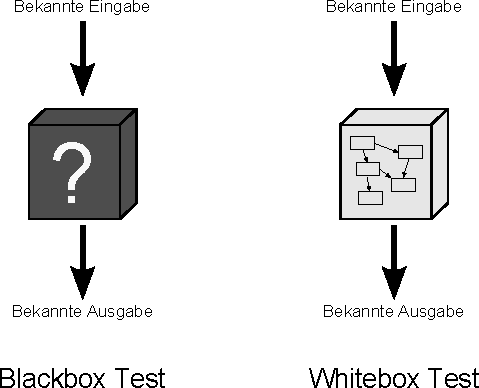
\includegraphics[width=.8\textwidth]{images/Qualitaetssicherung/abbildungen/BlackBoxAndWhiteBoxTesting}
  \end{center}
\end{frame}

%%%%%%%%%%%%%%%%%%%%%%%%%%%%%%%%%

\begin{frame}
\frametitle{Fuzzy Testing}
Fuzzing:
\begin{itemize}
	\item Unlike unit tests, fuzzy testing does not define test cases manually but generates them randomly based on statistic functions.
	\item By reaching a large number of generated tests, the software is tested for unusual values as well.
\begin{itemize}
	\item This is especially interesting for uncovering security relevant vulnerabilities.
\end{itemize}
\item Fuzzing is usually applied in black box testing to understand error affinity of new software and to detect vulnerabilities.
\item If a software reproducible generates a problem (e.g. crashes) under fuzzy testing, white box tests can be used to find the specific cause. 
\end{itemize}
\end{frame}

%%%%%%%%%%%%%%%%%%%%%%%%%%%%%%%%%

\begin{frame}
\frametitle{Test Oracle}
  \begin{center}
  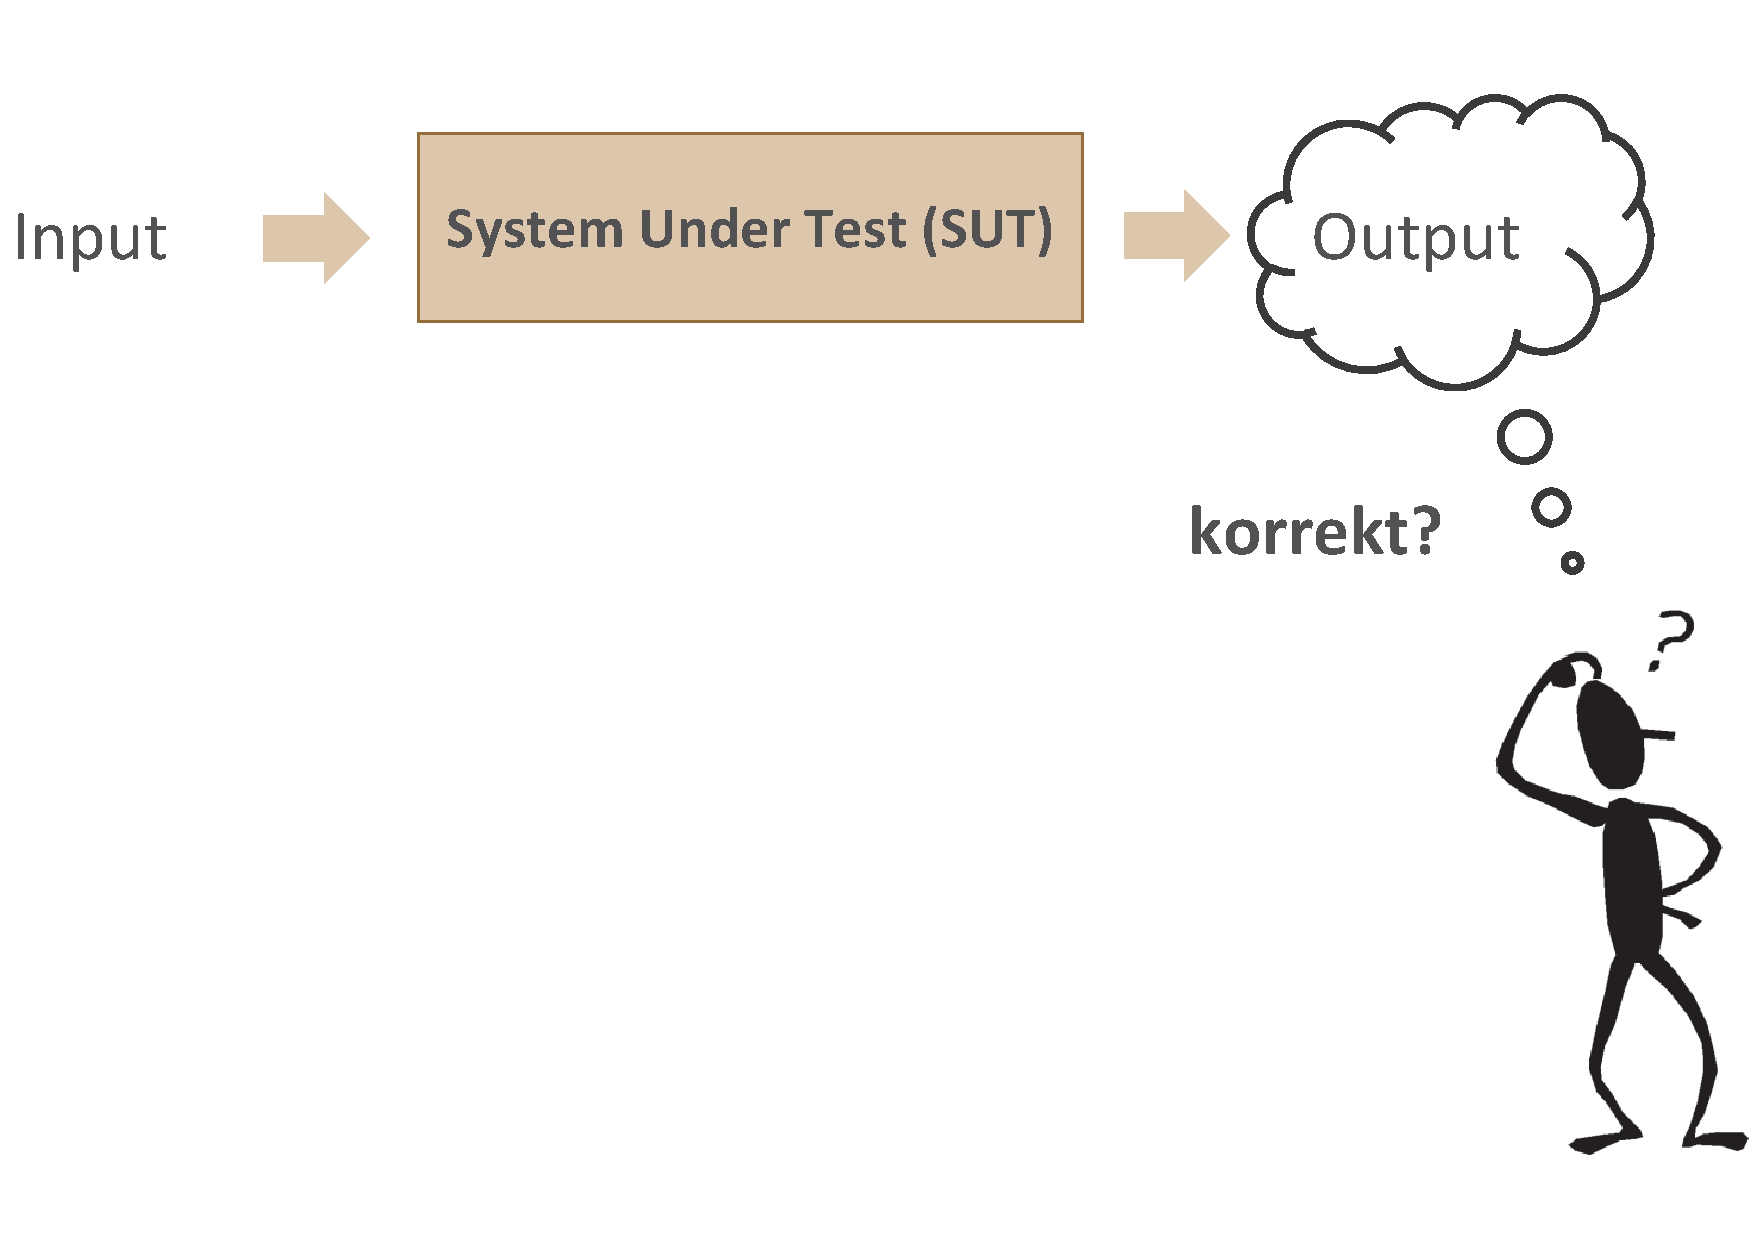
\includegraphics[width=\textwidth]{images/Qualitaetssicherung/abbildungen/TestOracle}
  \end{center}
\end{frame}

%%%%%%%%%%%%%%%%%%%%%%%%%%%%%%%%%

\begin{frame}
\frametitle{Are there types of software that do not have a test oracle}
  \begin{center}
  \url{https://monti.com}  % unreachable
  \end{center}
\end{frame}

%%%%%%%%%%%%%%%%%%%%%%%%%%%%%%%%%

\begin{frame}
\frametitle{The oracle problem}
\framesubtitle{It is not always possible to define a test oracle}
  \begin{center}
\only<beamer>{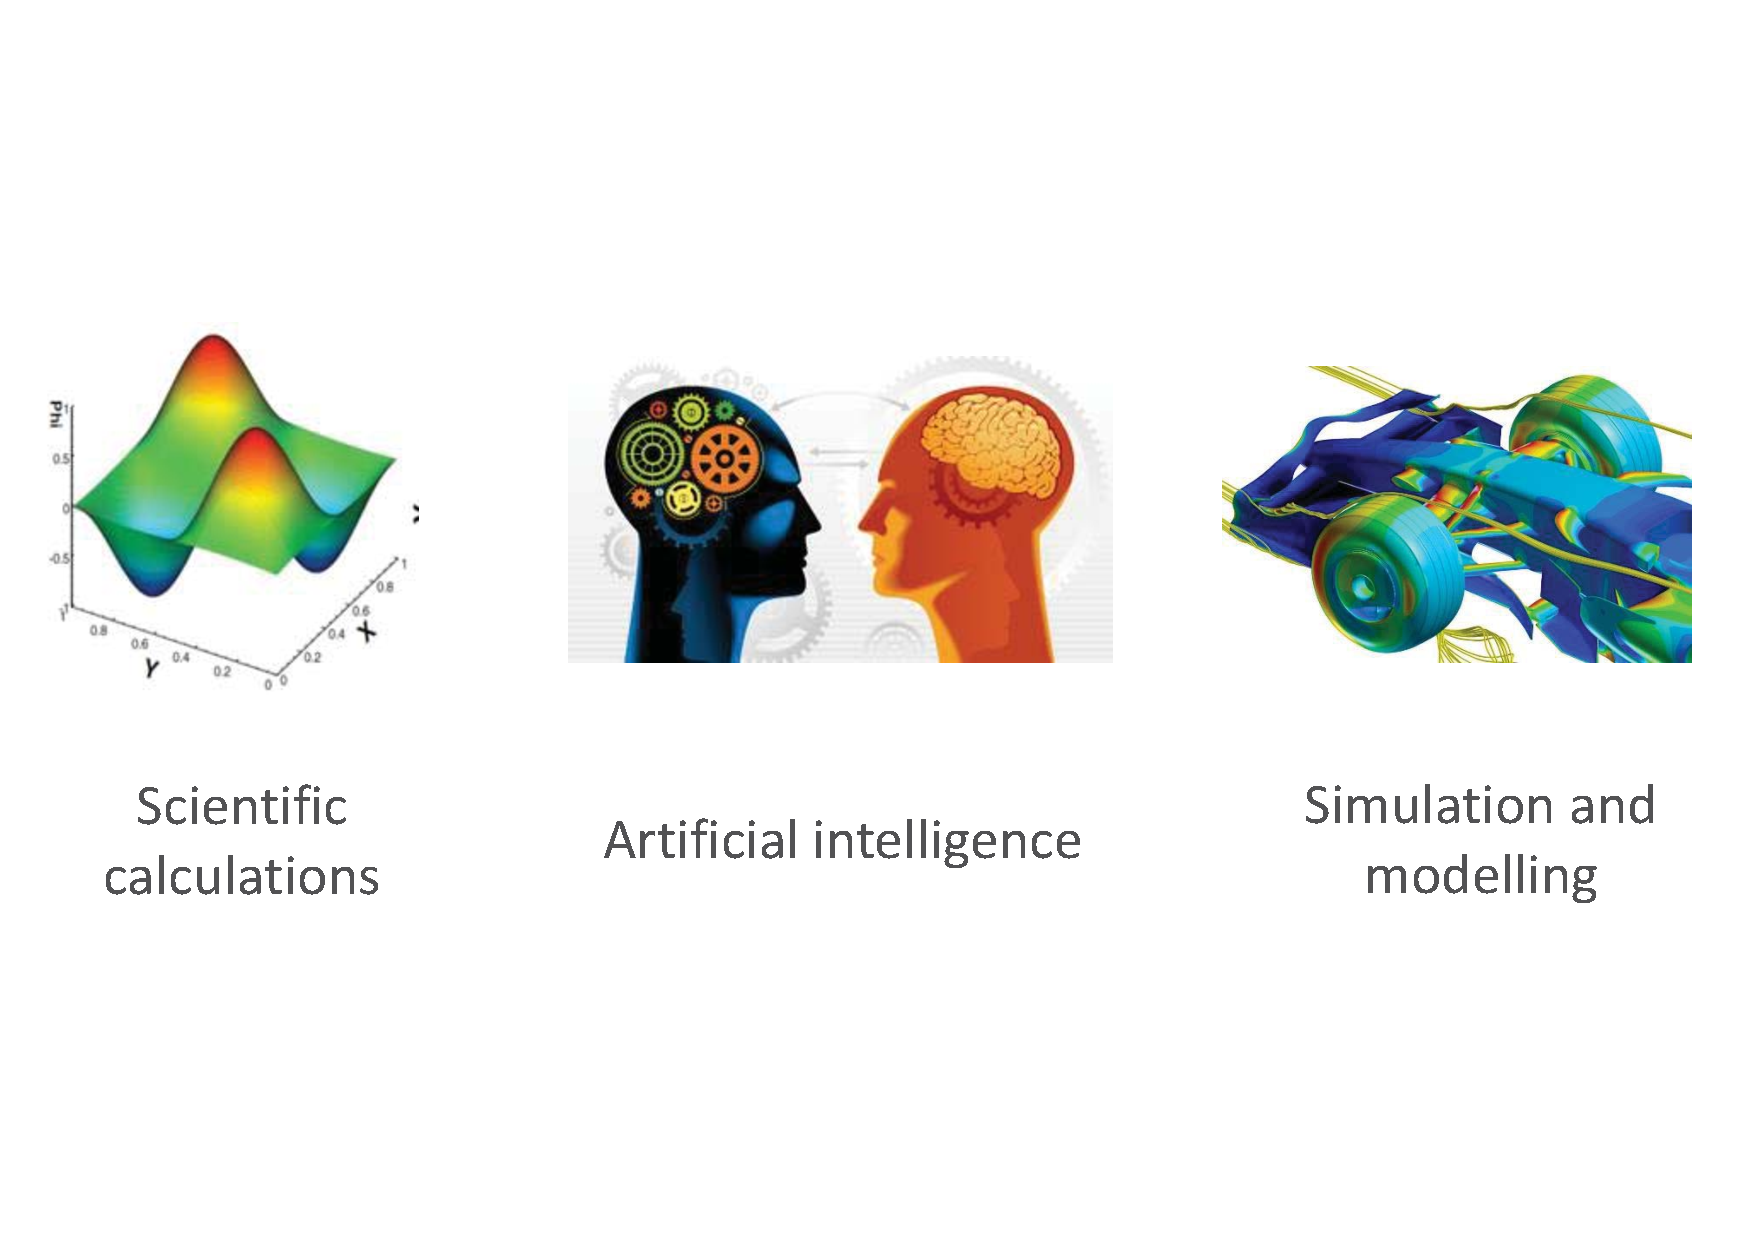
\includegraphics[width=\textwidth]{images/Qualitaetssicherung/abbildungen/TestOracleProblem}}
  \end{center}
	Was tun? \\
	%\citet{MetamorphicTesting2016,segura_metamorphic_2020,kanewala_metamorphic_2019}
\end{frame}

%%%%%%%%%%%%%%%%%%%%%%%%%%%%%%%%%

\begin{frame}
\frametitle{Application of metamorphic testing}
%\framesubtitle{\citet{segura_metamorphic_2020}}
  \begin{center}
  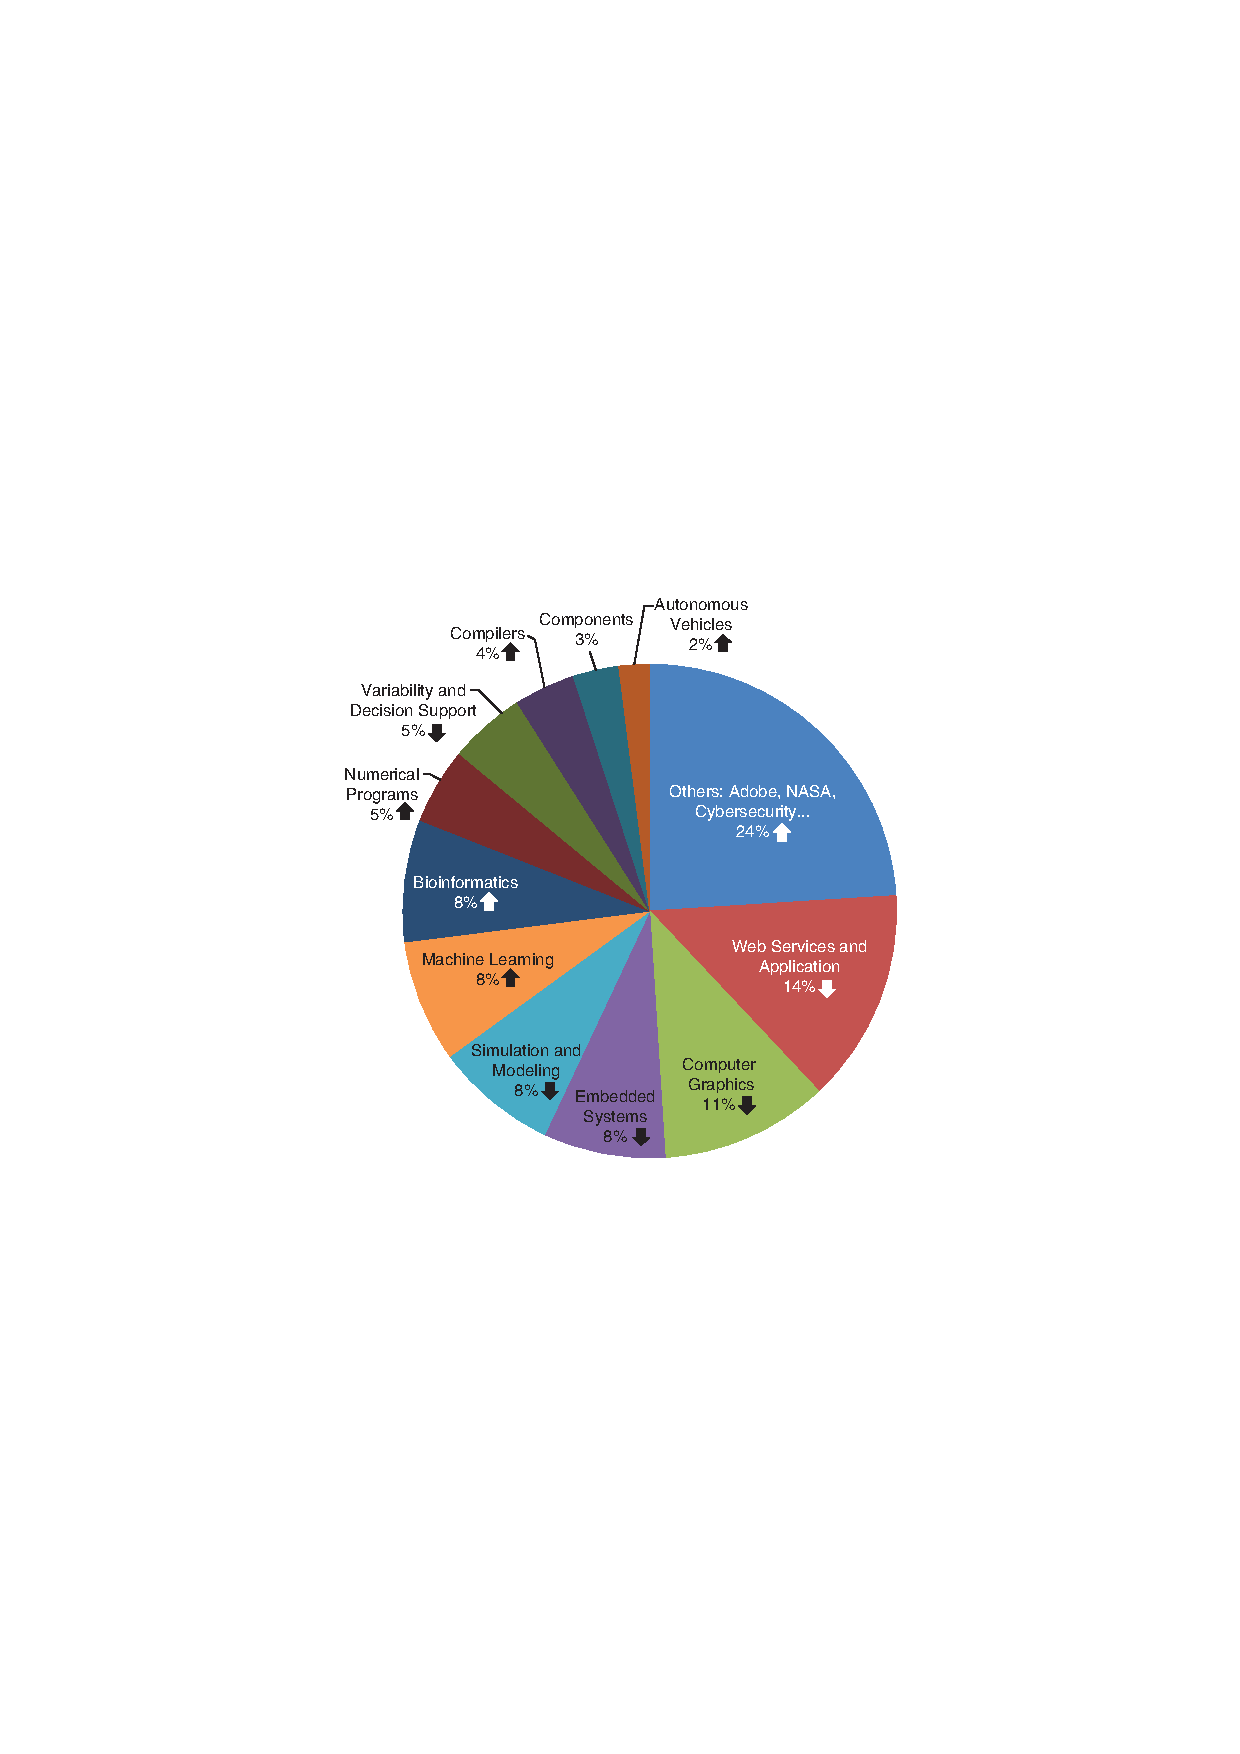
\includegraphics[width=.65\textwidth]{images/Qualitaetssicherung/abbildungen/MetamorphicTesting}
  \end{center}
\end{frame}


\mysubsubsection{Integrationstest}

%%%%%%%%%%%%%%%%%%%%%%%%%%%%%%%%%

\begin{frame}
\frametitle{Integrationstest}
\framesubtitle{Testing in the large}
\begin{itemize}
  \item Der Test einzelner Module garantiert nicht, dass die Zusammenarbeit korrekt funktioniert.
  \item Viele Module k�nnen gar nicht isoliert getestet werden.
  \item Also: Vorgehensweise zum Test komplexer Systeme (modulares Testen):
    \begin{itemize}
      \item Modultests (a.k.a.\ Unit Tests \&\ Components Tests)\\
			Testen eine Komponente ohne Kontext.
      \item Inkrementeller Integrationstest mehrer Komponenten im Kontext.
      \item Systemtest: Test des gesamten Systems in der Anwendungsumgebung (end-to-end).
    \end{itemize}
	\item Akzeptanztests (a.k.a.\ Funktionstests)\\
Focus auf das Testen von `cross-cutting' Funktionalit�t.
\end{itemize}
\end{frame}

%%%%%%%%%%%%%%%%%%%%%%%%%%%%%%%%%

\begin{frame}
\frametitle{Integrationstest (Forts.)}
\begin{itemize}
  \item Bei eingebetteten Realzeitsystemen muss auch das Zusammenspiel von Hard- und Software getestet werden.
	\begin{itemize}
		\item Digital Twins
	\end{itemize}
  \item Inkrementelles Testen ist dem \glq Big-Bang\grq-Testen, wobei nach den Modultests direkt das Gesamtsystem getestet wird, vorzuziehen.
  \item Die Trennung zwischen Schnittstelle und Implementierung erleichtert den Integrationstest erheblich.
    \begin{itemize}
      \item Leichtes Ersetzen von \glq Mockups\grq\ durch \glq richtige\grq\ Module.\\
			Siehe z.B.\ Mockito \url{https://github.com/mockito/}
    \end{itemize}
\end{itemize}
\end{frame}

%%%%%%%%%%%%%%%%%%%%%%%%%%%%%%%%%

\begin{frame}
\frametitle{Inkrementelles Testen}
\begin{center}
\pgfimage[width=0.9\textwidth]{Qualitaetssicherung/abbildungen/Inkrementelles_Testen}\\
"`Testger�st"'
\end{center}
 
\begin{itemize}
	\item Inkrementelle Tests k�nnen entsprechend den Benutzt- und Kompositions-Hierarchien bottom-up oder top-down erfolgen; nat�rlich auch jo-jo. 
	\item Eine hierarchische Architektur ist dabei sehr f�rderlich.
\end{itemize}
\end{frame}

\mysubsubsection{Regression testing }

%%%%%%%%%%%%%%%%%%%%%%%%%%%%%%%%%

\begin{frame}
\frametitle{Regression testing}
\begin{itemize}
  \item A test tool saves all test cases that have been done.
  \item This allows for an automatic repretition of all past tests after the software under test was changed.
  \item Executes nominal-actual comparison:
    \begin{itemize}
      \item Input data for the test object
      \item Expected outputs or reactions of test object
    \end{itemize}
\end{itemize}
\end{frame}

%%%%%%%%%%%%%%%%%%%%%%%%%%%%%%%%%

%\begin{frame}
%\frametitle{Test Driven Development}
%\framesubtitle{Testgetriebene Entwicklung}
    %\begin{itemize}
    %\item Martin Fowler:\\
        %``Whenever you are tempted to type something into a print statement or a debugger expression, write it as a test instead.''
    %\item ``One of the ironies of Test Driven Development is that it isn't a testing technique. It's an analysis technique, a design technique, really a technique structuring all the activities of development.'' \cite{Beck2002}.                  
          %
    %\item Testen als Spezifikation und Entwurfsmittel.
          %
    %\item Tests sind eine Form von ausf�hrbarer Dokumentation.
          %
    %\item Regressionstests sind ein n�tzlicher Nebeneffekt.
          %
    %\end{itemize}
%\end{frame}

%%%%%%%%%%%%%%%%%%%%%%%%%%%%%%%%%

%\begin{frame}
%\frametitle{Werkzeugunterst�tzung zum Testen}
%\framesubtitle{Unit- und Integrations-Tests}
%\begin{itemize}
  %\item JUnit ist ein Testwerkzeug f�r Java \citep{Link2002}\\
    %(\url{http://www.junit.org/}).
	%\item Selenium-Integrations-Tests f�r Browser (\url{http://seleniumhq.org/}).
	%\item testIT WebTester als UI-Testautomatisierungs-Framework f�r Web-Applikationen basierend auf Selenium (\url{https://www.novatec-gmbh.de/produkte/testit-webtester/}).
%\end{itemize}
%Unit-Tests und Integrations-Tests sind mit diesen Werkzeugen automatisch wiederholbar.
%\end{frame}

%%%%%%%%%%%%%%%%%%%%%%%%%%%%%%%%%

%\begin{frame}
%\frametitle{Automatisierte Akzeptanztests}
%\framesubtitle{\citep{FIT2005,FIT2006}}
%\begin{itemize}
  %\item Die zu pr�fende Gesch�ftslogik und die erwarteten
    %Testergebnisse werden in Tabellenform dargestellt (HTML), so dass auch
    %Fachexperten an der Erstellung und Durchf�hrung der Tests
    %teilnehmen k�nnen.
  %\item FIT (Framework for Integrated Test) ist ein Werkzeug,
    %welches automatisierte und wiederholbare Akzeptanztests erlaubt
    %(\url{http://fit.c2.com/})
	%\item FitNesse erg�nzt FIT u.a.\ um ein Wiki zur kollaborativen Erstellung von Akzeptanztests (\url{http://www.fitnesse.org/})
%\end{itemize}
%\end{frame}

%%%%%%%%%%%%%%%%%%%%%%%%%%%%%%%%%

\begin{frame}
\frametitle{Test driven development and refactoring}
\begin{itemize}
  \item Test driven development combines two techniques: 
    \begin{itemize}
      \item Test-driven programming for external evolution,
      \item refactoring for internal evolution.
    \end{itemize}
  \item Refactoring\\
        Changing a program with the aim of improving the internal structure without changing the (external) functionality.
  \item Refactoring is allowed if all tests are passing.
  \item Here, tests are a form of executable specification.
\end{itemize}
\end{frame}

%%%%%%%%%%%%%%%%%%%%%%%%%%%%%%%%%

\begin{frame}
\frametitle{Continuous Integration}
Aims for (among others):
\begin{itemize}
	\item Execution of static analyses (e.g., SpotBugs, Checkstyle)
	\item Building the systems (e.g., Gradle)
	\item Automated execution of tests (e.g.\ JUnit, Selenium) \citep{TestAutomation2013}
	\item Checking of log and monitoring data (e.g.\ Kieker) \citep{SEN2015}
\end{itemize}
\end{frame}

%%%%%%%%%%%%%%%%%%%%%%%%%%%%%%%%%

\begin{frame}
\frametitle{DevOps: Development and operations}
\framesubtitle{Continuous Testing, Delivery \&\ Deployment}
\begin{center}
\pgfimage[width=0.7\textwidth]{Qualitaetssicherung/abbildungen/DevOps2016}
\end{center}
\end{frame}

%%%%%%%%%%%%%%%%%%%%%%%%%%%%%%%%%

\begin{frame}
\frametitle{Agility and reliability}
\framesubtitle{By Continuous Testing, Example otto.de \citep{ICSA2017}}
\begin{center}
\pgfimage[width=\textwidth]{Qualitaetssicherung/abbildungen/DeploymentIncidentsBars}
\end{center}
\end{frame}


%%
%\backupbegin
%\section{References}

%%%%%%%%%%%%%%%%%%%%%%%%%%%%%%%%%
%\begin{frame}[t,allowframebreaks]{References}
%  \frametitle{\bibname}
%  \printbibliography
%\end{frame}

%\backupend

\end{document}
